\paragraph{}
	L'interface graphique sera codée en C++ et respectera le modèle MVC. \\
	Ainsi seul le contrôleur modifiera le modèle, tandis que la classe NoSkin, représentant l'interface,
	ne fera qu'afficher les données. \\
	Ces deux classes sont donc représentées sur l'UML et sont complémentées par des classes complémentaires
	telles que la classe FormatException qui permet de gérer plus finement la conversion JSON/Objet.\\
	Les classes TabWidget, Options et Chord seront utilisées par NoSkin pour créer les fenêtres de 
	l'accordeur, des paramètres et le widget particulier de la tablature.

\begin{figure}[H]

	\centering 
	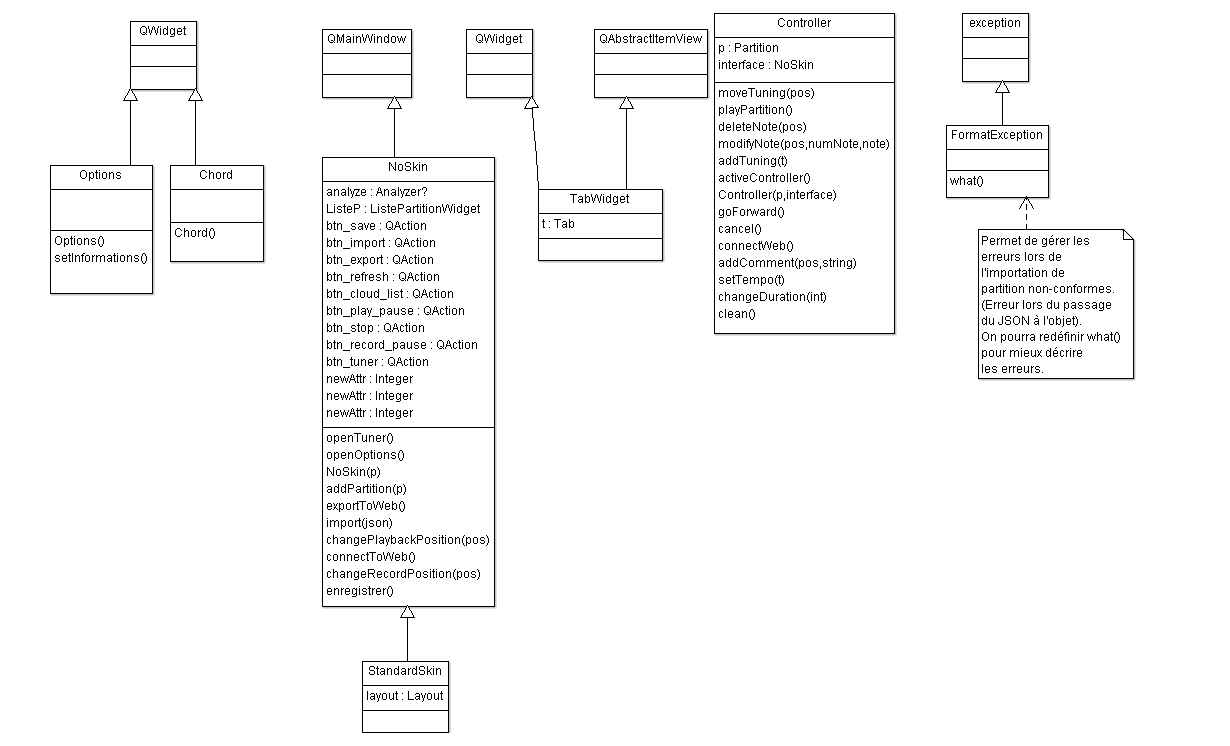
\includegraphics[scale=0.3]{GUI_UML}
		\caption{UML de l'interface graphique}
			

\end{figure}

